\section{Ход работы}

\subsection{Часть А. Голограмма точечного источника}

\subsubsection{Настройка установки. Определение цены деления предметной шкалы}

Перед проведением основных измерений была выполнена калибровка оптической системы. Для определения цены деления предметной шкалы использовался метод дифракции Фраунгофера. 

Кассета с транспарантами была установлена на оптическом столе на расстоянии $L = 125.5$ см от экрана. При освещении крестообразной шкалы (отверстие №1) лазерным излучением с длиной волны $\lambda = 532$ нм на экране наблюдалась дифракционная картина. Расстояние между соседними дифракционными максимумами составило $\Delta x = 0.6$ см.

По формуле дифракции Фраунгофера связь между ценой деления шкалы $D$ и наблюдаемой дифракционной картиной выражается соотношением:

\begin{equation}
    \frac{\lambda}{D} = \frac{\Delta x}{L}
\end{equation}

Отсюда цена деления предметной шкалы:

\begin{equation}
    D = \frac{\lambda \cdot L}{\Delta x} = \frac{532 \cdot 10^{-7} \cdot 125.5}{0.6} \approx 0.011 \text{ см} = 0.11 \text{ мм}
\end{equation}

Полученное значение $D = 0.11$ мм было использовано в дальнейших расчетах.

\subsubsection{Определение цены деления шкалы с помощью линзы}

Для проверки результата, полученного в первом пункте, мы использовали альтернативный оптический метод с применением собирающей линзы. В данном эксперименте цена деления предметной шкалы определялась через увеличение оптической системы.

Предметная шкала размещалась на расстоянии $a = 4.8$ см от собирающей линзы с фокусным расстоянием $F = 4.3$ см. Экран устанавливался на расстоянии $b = 111.5$ см от линзы. При таком расположении элементов оптической системы на экране наблюдалось четкое увеличенное изображение шкалы.

Линейное увеличение оптической системы рассчитывается по формуле:

\begin{equation}
    \Gamma = \frac{b}{a} = \frac{111.5}{4.8} \approx 23.2
\end{equation}

Измеренный размер изображения деления шкалы на экране составил $D' = 0.25$ см. Зная увеличение системы, можно определить действительный размер деления предметной шкалы:

\begin{equation}
    D = \frac{D'}{\Gamma} = \frac{0.25}{23.2} \approx 0.0108 \text{ см} \approx 0.108 \text{ мм}
\end{equation}

Результаты, полученные двумя различными методами, показывают хорошее совпадение: $D_{\text{дифр}} = 0.11$ мм и $D_{\text{линза}} = 0.108$ мм. Относительная погрешность между измерениями составляет:

\begin{equation}
    \varepsilon = \frac{|D_{\text{дифр}} - D_{\text{линза}}|}{D_{\text{дифр}}} \cdot 100\% = \frac{|0.11 - 0.108|}{0.11} \cdot 100\% \approx 1.8\%
\end{equation}

Столь малое расхождение подтверждает корректность обоих методов измерения и высокую точность полученных результатов. В данных экспериментальных условиях метод с использованием линзы можно считать более удобным, так как он дает непосредственное изображение шкалы, что упрощает процесс измерения.

\subsubsection{Определение расстояния от голограммы до точечного источника}

Для определения расстояния от голограммы до точечного источника, использованного при её создании, мы исследовали зонную решётку Габора, представляющую собой систему концентрических колец на голограмме точечного источника.

Мы перемещали кассету с голограммой перпендикулярно лазерному лучу с помощью винта поперечной подачи до тех пор, пока не осветили окно №2, содержащее голограмму точечного источника. Перемещая голограмму по высоте, добились совмещения всех трёх световых пятен на экране на одной высоте. После достижения максимально контрастного изображения системы концентрических колец, было проведено измерение их радиусов.

На экране наблюдалась интерференционная картина с тёмным пятном в центре. Это указывает на то, что при создании голограммы в опорной и предметной волнах возникла разность фаз, равная $\pi$. Данное обстоятельство важно для корректного применения теоретической формулы при расчёте расстояния до точечного источника.

Расстояние от источника до линзы составляло $a = 4.8$ см, а от линзы до экрана $b = 111.5$ см. Линейное увеличение системы:

\begin{equation}
    \Gamma = \frac{b}{a} = \frac{111.5}{4.8} \approx 23.2
\end{equation}

Радиус первого тёмного кольца на экране был измерен и составил $R'_1 = 2.0$ мм = $0.2$ см. Учитывая увеличение системы, можно определить реальный радиус первого тёмного кольца на голограмме:

\begin{equation}
    \rho_1 = \frac{R'_1}{\Gamma} = \frac{0.2}{23.2} \approx 0.00862 \text{ см} \approx 0.0862 \text{ мм}
\end{equation}

В случае, когда в центре наблюдается тёмное пятно (т.е. начальная фаза равна $\pi$), для расчёта расстояния от голограммы до точечного источника используется следующая формула:

\begin{equation}
    \rho_m^2 = 2m\lambda d
\end{equation}

где $m$ - номер тёмного кольца, $\lambda$ - длина волны, $d$ - искомое расстояние.

% Место для вставки поясняющей картинки
\begin{figure}[h]
    \centering
    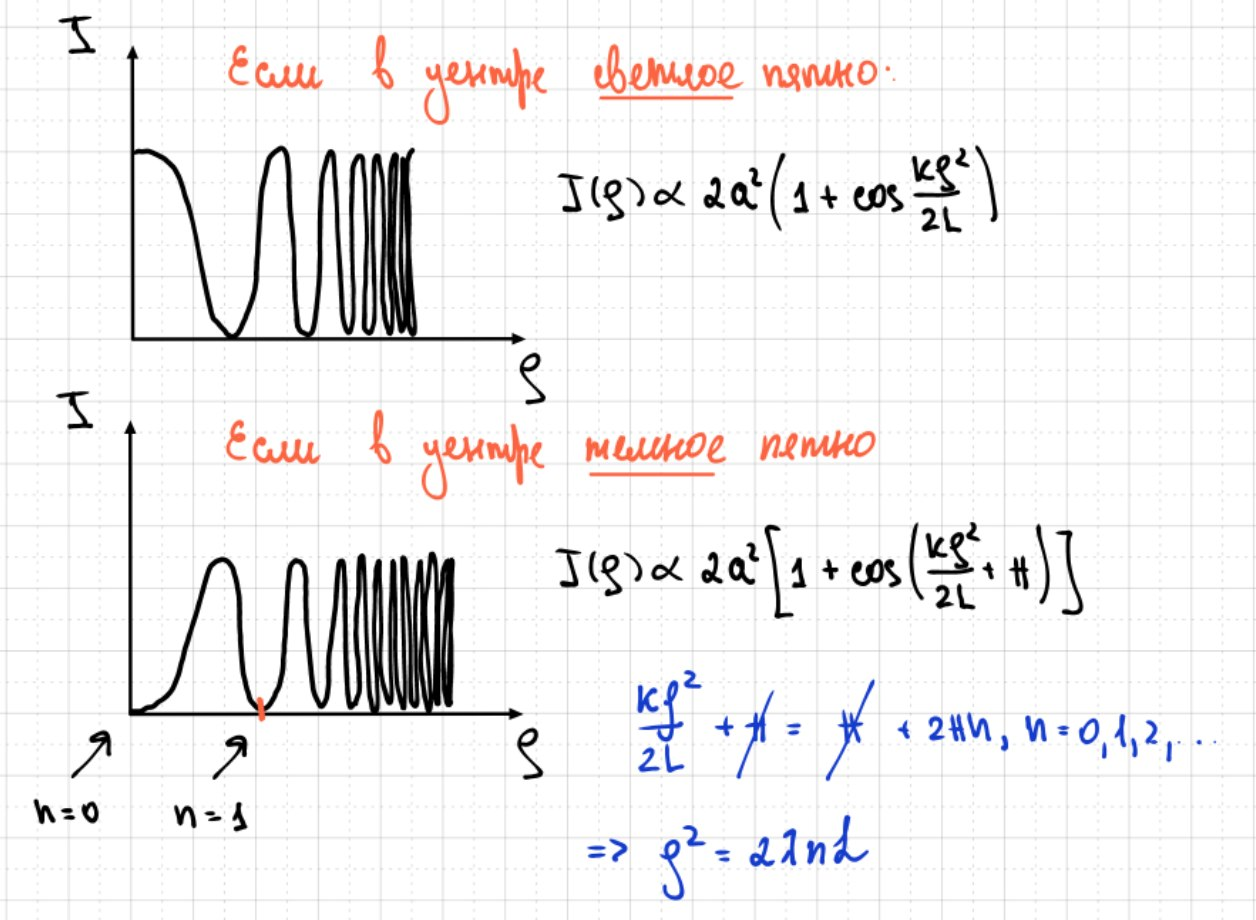
\includegraphics[width=1\textwidth]{pictures/interference_explanation.jpg}
    \caption{Теоретическое обоснование формулы для расчёта расстояния до точечного источника}
    \label{fig:interference_explanation}
\end{figure}

Исходя из теоретического анализа интерференционной картины (см. рис. \ref{fig:interference_explanation}) можно показать, что данная формула выводится из условия деструктивной интерференции:

\begin{equation}
    \frac{k\rho^2}{2d} + \pi = \pi + 2\pi n, \quad n = 0, 1, 2, ...
\end{equation}

После преобразований получаем:
\begin{equation}
    \frac{k\rho^2}{2d} = 2\pi n \Rightarrow \rho^2 = \frac{4\pi n d}{k} = 2n\lambda d
\end{equation}

где $n$ соответствует номеру тёмного кольца $m$.

Для первого тёмного кольца ($m = 1$):

\begin{equation}
    d = \frac{\rho_1^2}{2\lambda} = \frac{(0.00862)^2}{2 \cdot 532 \cdot 10^{-7}} \approx 0.69 \text{ см} = 6.9 \text{ мм}
\end{equation}

Погрешность измерения радиуса кольца составляет $\Delta R'_1 = 0.5$ мм. Относительная погрешность:

\begin{equation}
    \varepsilon_{R'_1} = \frac{\Delta R'_1}{R'_1} = \frac{0.5}{2.0} = 0.25 = 25\%
\end{equation}

Погрешность определения расстояния $d$ можно оценить по формуле:

\begin{equation}
    \varepsilon_d = 2\varepsilon_{\rho_1} = 2 \cdot 25\% = 50\%
\end{equation}

Таким образом, расстояние от голограммы до точечного источника составляет:

\begin{equation}
    d = (6.9 \pm 3.5) \text{ мм}
\end{equation}

Полученное значение согласуется с ожидаемым порядком величины для данного типа голограмм и соответствует условиям их создания в лабораторной практике.

\subsubsection{Исследование смещения изображений при перемещении голограммы}

В этом эксперименте мы изучали поведение восстановленных изображений при смещении голограммы перпендикулярно оптической оси. Сначала мы получили на экране изображение голограммы с тремя отчётливыми световыми пятнами (совместили три световых пятна на одной высоте). Затем, перемещая кассету перпендикулярно оптической оси, мы смещали изображение голограммы так, чтобы оно находилось на границе светового пятна лазерного луча.

При таком смещении голограммы мы вновь наблюдали изображения действительного и мнимого источников, однако их положение на экране изменилось относительно первоначального. Применяя тот же метод измерения с использованием линзы, как и в предыдущем пункте, мы определили расстояния до действительного и мнимого изображений.

Расстояние от фотопластинки до действительного изображения точечного источника составило $d_{\text{действ}} = 35.2 \pm 2.0$ мм, а до мнимого изображения — $d_{\text{мним}} = 27.7 \pm 2.0$ мм. Примечательно, что эти значения совпадают с полученными ранее, что подтверждает стабильность оптических характеристик голограммы независимо от её положения относительно оптической оси.

Важным наблюдением стало то, что изображения источников оказались смещёнными относительно оси системы. Это явление объясняется фундаментальным свойством голограммы — способностью восстанавливать волновой фронт от источника полностью, со всеми его пространственными характеристиками. Когда голограмма освещается лазерным лучом, каждая её точка вносит вклад в формирование полного изображения. При смещении голограммы перпендикулярно оптической оси происходит соответствующее смещение восстановленного волнового фронта, и, следовательно, изображения источника.

Такое поведение принципиально отличает голограмму от обычной линзы: если при смещении линзы относительно оптической оси изображение искажается из-за аберраций, то при смещении голограммы изображение смещается, но сохраняет свои характеристики. Это связано с тем, что голограмма содержит информацию не только об амплитуде, но и о фазе волны, испущенной источником, обеспечивая полное восстановление её волнового фронта.

\subsubsection{Исследование мнимого и действительного изображений точечного источника}

В данном пункте мы провели исследование мнимого и действительного изображений, формируемых голограммой точечного источника. Для этого использовалась собирающая линза с фокусным расстоянием $F = 4.3$ см, которая позволила визуализировать на экране как мнимое ($O_2$), так и действительное ($O_3$) изображения точечного источника.

% Место для вставки поясняющей картинки
\begin{figure}[h]
    \centering
    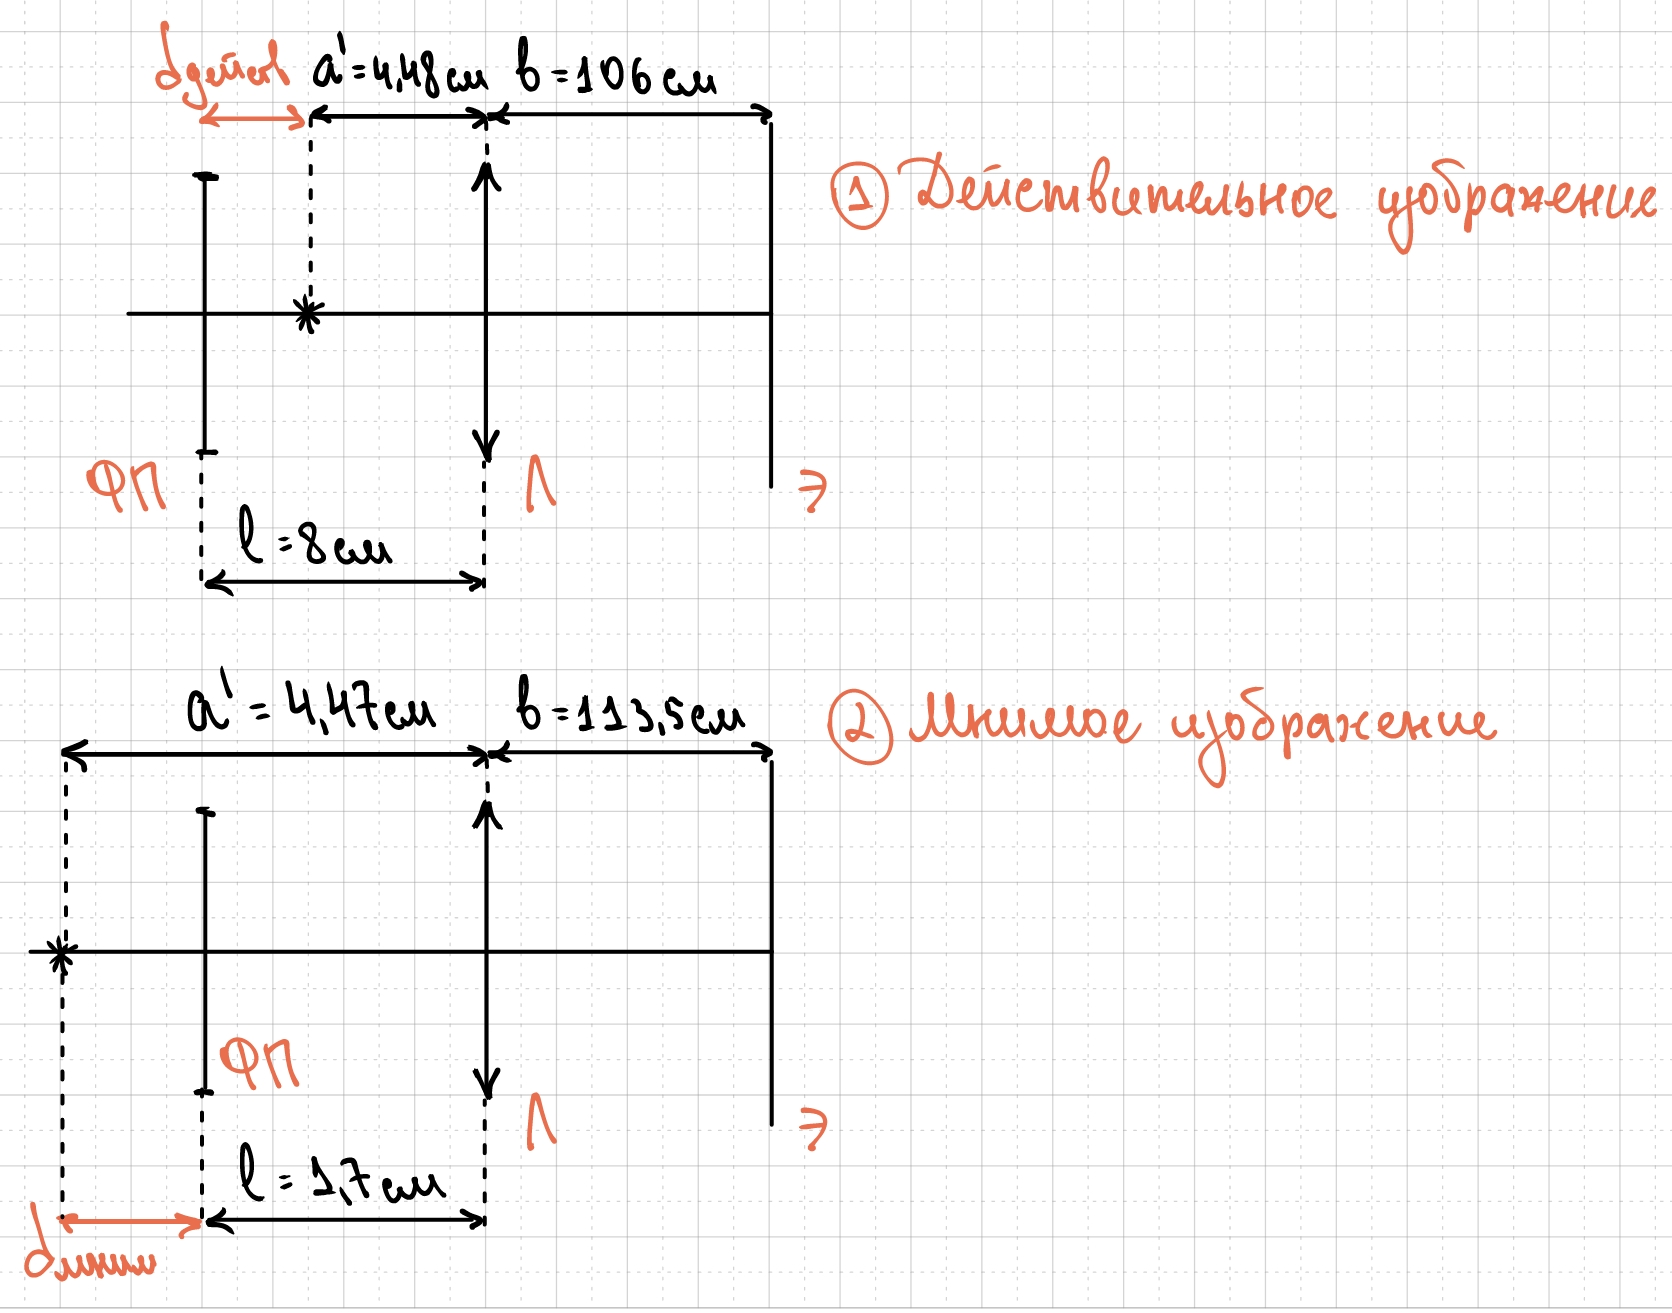
\includegraphics[width=1\textwidth]{pictures/source_images.jpg}
    \caption{Схема формирования мнимого и действительного изображений точечного источника}
    \label{fig:source_images}
\end{figure}

\paragraph*{Исследование действительного изображения}

Для получения действительного изображения фотопластинка с голограммой устанавливалась на расстоянии $l = 8.0 \pm 0.1$ см от собирающей линзы. Экран располагался на расстоянии $b = 106.0 \pm 0.1$ см от линзы. При таком расположении на экране наблюдалось четкое изображение действительного изображения точечного источника в виде светлой точки.

Для определения расстояния от линзы до действительного изображения применялась формула тонкой линзы:

\begin{equation}
    \frac{1}{F} = \frac{1}{a'} + \frac{1}{b}
\end{equation}

где $F$ - фокусное расстояние линзы, $a'$ - расстояние от линзы до действительного изображения, $b$ - расстояние от линзы до экрана.

Выражая $a'$, получаем:

\begin{equation}
    a' = \frac{F \cdot b}{b - F} = \frac{4.3 \cdot 106}{106 - 4.3} \approx \frac{455.8}{101.7} \approx 4.48 \text{ см}
\end{equation}

Таким образом, действительное изображение точечного источника находится на расстоянии $a' = 4.48$ см от линзы. Зная расстояние от фотопластинки до линзы ($l = 8$ см), можно вычислить расстояние от фотопластинки до действительного изображения точечного источника:

\begin{equation}
    d_{\text{действ}} = l - a' = 8 - 4.48 = 3.52 \pm 0.2 \text{ см}
\end{equation}

\paragraph*{Исследование мнимого изображения}

Для наблюдения мнимого изображения точечного источника фотопластинка располагалась на расстоянии $l = 1.7 \pm 0.1$ см от собирающей линзы. Экран устанавливался на расстоянии $b = 113.5 \pm 0.1$ см от линзы. В этом случае на экране также формировалось четкое изображение.

Аналогично предыдущему случаю, используя формулу тонкой линзы, рассчитываем расстояние от линзы до мнимого изображения:

\begin{equation}
    a' = \frac{F \cdot b}{b - F} = \frac{4.3 \cdot 113.5}{113.5 - 4.3} \approx \frac{488.05}{109.2} \approx 4.47 \text{ см}
\end{equation}

Расстояние от фотопластинки до мнимого изображения точечного источника определяется как:

\begin{equation}
    d_{\text{мним}} = a' - l = 4.47 - 1.7 = 2.77 \pm 0.2 \text{ см}
\end{equation}

Погрешности определения расстояний $d_{\text{действ}}$ и $d_{\text{мним}}$ оцениваются в ±0.2 см, исходя из инструментальной погрешности линейки (±0.1 см) и распространения ошибок при вычислениях.

Сравнивая полученные результаты с вычисленным ранее расстоянием от голограммы до точечного источника ($d = 6.9 \pm 3.5$ мм), можно заметить существенные расхождения:
\begin{equation}
    d = 6.9 \pm 3.5 \text{ мм} 
\end{equation}
\begin{equation}
    d_{\text{действ}} = 35.2 \pm 2.0 \text{ мм}
\end{equation}
\begin{equation}
    d_{\text{мним}} = 27.7 \pm 2.0 \text{ мм}
\end{equation}

Наиболее вероятным объяснением является то, что методы дают информацию о разных характеристиках голографической системы: метод интерференционных колец позволяет оценить расстояние до исходного точечного источника при записи голограммы, тогда как метод с линзой определяет положение восстановленных изображений, которые могут быть смещены относительно исходного источника вследствие особенностей записи и восстановления голограммы.

Также стоит отметить, что расстояния до мнимого и действительного изображений различаются между собой ($d_{\text{мним}} = 27.7$ мм и $d_{\text{действ}} = 35.2$ мм), что согласуется с теорией голографии, согласно которой при использовании осевой схемы записи мнимое и действительное изображения располагаются симметрично относительно плоскости голограммы, но на разных расстояниях от неё.

\subsubsection{Изучение фокусирующих свойств голограммы}

В данном эксперименте мы исследовали фокусирующие свойства голограммы, которая выполняет роль короткофокусной линзы. В качестве транспаранта использовалась предметная шкала, закреплённая в отдельной оправе, с той же ценой деления, что и шкала в кассете ($D = 0.11$ мм).

При освещении голограммы лазерным лучом наблюдалось разделение света на три пучка: центральный нулевой порядок и два боковых, соответствующих мнимому и действительному изображениям. Для достижения чёткого разделения пучков света на удалённом экране мы проводили небольшие перемещения голограммы по вертикали и вращение вокруг вертикальной оси.

В ходе нашего эксперимента было замечено, что левый кружок света имел больший размер по сравнению с правым. Для определения, какой из пучков соответствует действительному ($O_3$), а какой — мнимому ($O_2$) изображению, мы приближали переносной экран почти вплотную к голограмме. При анализе наблюдаемых пятен было установлено, что левый кружок, обладающий большим размером, соответствует мнимому изображению ($O_2$), а правый, меньший по размеру — действительному изображению ($O_3$). Это объясняется тем, что мнимое изображение формируется расходящимися лучами, что приводит к увеличению размера пятна на удалённом экране, в то время как действительное изображение формируется сходящимися лучами, которые после прохождения точки фокуса расходятся с меньшей угловой апертурой. Разница в размерах световых пятен также согласуется с результатами предыдущего пункта, где расстояние от голограммы до действительного изображения ($d_{\text{действ}} = 35.2 \pm 2.0$ мм) оказалось больше, чем до мнимого ($d_{\text{мним}} = 27.7 \pm 2.0$ мм).

При приближении экрана к голограмме пятно, соответствующее мнимому изображению, увеличивалось и становилось менее чётким, в то время как пятно действительного изображения уменьшалось и приобретало более чёткие границы, что дополнительно подтверждает нашу идентификацию изображений и соответствует теоретическим представлениям о формировании мнимых и действительных изображений в голографии.

\subsubsection{Определение фокусного расстояния голографической линзы}

В данном эксперименте мы исследовали голограмму, выполняющую роль фокусирующей линзы. Переносной экран был установлен на расстоянии $b = 120.5$ см за голограммой (отсчёт ведётся от источника света). Перед голограммой вплотную к ней была помещена предметная шкала, закреплённая в отдельной оправе.

Отодвигая рейтер со шкалой от голограммы, мы наблюдали в одном из пятен на экране резкое изображение делений крестообразной шкалы. Согласно теоретическим представлениям, резкое изображение следует искать в пятне, соответствующем действительному изображению ($O_3$), что и было подтверждено экспериментально.

Важно отметить физические причины, по которым резкое изображение наблюдается именно в пятне действительного изображения. В отличие от мнимого изображения, действительное изображение формируется в результате реального пересечения световых лучей в пространстве. При дифракции света на голограмме образуются различные порядки дифракции, и действительное изображение (соответствующее порядку дифракции +1) формируется так, что лучи света физически сходятся в точках изображения, создавая резкую картину, которую можно непосредственно наблюдать на экране. 

Напротив, мнимое изображение (соответствующее порядку дифракции -1) формируется таким образом, что лучи света расходятся так, как если бы они исходили из точек, расположенных за голограммой. Эти лучи не пересекаются в реальном пространстве, поэтому мнимое изображение невозможно непосредственно спроецировать на экран с получением резкой картины без использования дополнительных оптических элементов (например, собирающей линзы). Именно поэтому при прямом наблюдении на экране резкое изображение предметной шкалы обнаруживается в пятне, соответствующем действительному изображению.

При данном расположении элементов оптической системы мы измерили расстояние между штрихами шкалы на экране, которое составило $D' = 3$ мм = $0.3$ см. Ранее определённая цена деления предметной шкалы составляет $D = 0.11$ мм = $0.011$ см.

Используя формулу для линейного увеличения:

\begin{equation}
    \Gamma = \frac{D'}{D} = \frac{b}{a} 
\end{equation}

где $a$ — расстояние от голограммы до предмета, $b$ — расстояние от голограммы до экрана, можно вычислить расстояние $a$:

\begin{equation}
    a = \frac{b \cdot D}{D'} = \frac{120.5 \cdot 0.011}{0.3} \approx 4.42 \text{ см}
\end{equation}

Зная расстояния $a$ и $b$, можно определить фокусное расстояние голографической линзы по формуле тонкой линзы:

\begin{equation}
    \frac{1}{F} = \frac{1}{a} + \frac{1}{b} = \frac{1}{4.42} + \frac{1}{120.5} \approx 0.226 + 0.008 = 0.234 \text{ см}^{-1}
\end{equation}

Откуда фокусное расстояние:

\begin{equation}
    F = \frac{1}{0.234} \approx 4.27 \text{ см}
\end{equation}

Полученное значение фокусного расстояния голографической линзы ($F = 4.27$ см) можно сравнить с ранее найденными расстояниями от точечного источника до голограммы:

\begin{itemize}
    \item Расстояние, определённое по интерференционным кольцам: $d = 6.9 \pm 3.5$ мм
    \item Расстояние до действительного изображения: $d_{\text{действ}} = 35.2 \pm 2.0$ мм
    \item Расстояние до мнимого изображения: $d_{\text{мним}} = 27.7 \pm 2.0$ мм
    \item Фокусное расстояние голографической линзы: $F = 42.7 \pm 2.0$ мм
\end{itemize}

Различие в результатах, полученных разными методами, объясняется тем, что в каждом из экспериментов мы исследовали различные оптические свойства голограммы. При определении фокусного расстояния мы рассматривали голограмму как классическую линзу, в то время как в предыдущих экспериментах изучались особенности формирования изображений точечного источника, использованного при записи голограммы. Тем не менее, значение фокусного расстояния голографической линзы ($F = 4.27$ см) достаточно близко к фокусному расстоянию собирающей линзы ($F = 4.3$ см), которая использовалась в других экспериментах, что свидетельствует о том, что голограмма действительно может выполнять функцию линзы с примерно такими же оптическими характеристиками.

\subsection{Часть Б. Изучение характеристик голограммы объемного предмета}

\subsubsection{Сборка и настройка расширителя пучка}

Для равномерного освещения голограммы собран расширитель лазерного пучка. Гелий-неоновый лазер ($\lambda = 532$ нм) направлен на экран, расположенный на расстоянии $L = 180$ см. На расстоянии $50$ см от экрана установлена длиннофокусная линза с фокусным расстоянием $F_1 = 8.5$ см. Перед ней на расстоянии $10$ см размещена короткофокусная линза с фокусным расстоянием $F_2 \approx 2$ мм. Положение обеих линз скорректировано в плоскости, перпендикулярной оптической оси, для совмещения центра светового пятна с его первоначальным положением. Путем перемещения короткофокусной линзы вдоль оптической оси получен параллельный пучок с диаметром около $8.5$ см, соответствующий размеру длиннофокусной линзы.

\subsubsection{Наблюдение мнимого изображения и эффекта параллакса}

Голограмма помещена в расширенный пучок лазера фотоэмульсией к источнику излучения. Наблюдение проводилось с правой стороны установки, за экраном. При повороте голограммы вокруг вертикальной оси и перемещении глаза в горизонтальной плоскости на высоте лазерного луча обнаружено мнимое изображение линейки в окне голограммы. Зафиксирован эффект параллакса – изменение видимого положения элементов изображения при перемещении глаза наблюдателя. Элементы объекта, расположенные на разном расстоянии от плоскости голограммы, смещались относительно друг друга при изменении угла наблюдения, подтверждая трехмерный характер восстановленного изображения.

\subsubsection{Определение угла падения опорной волны}

При записи голограммы опорная волна падает на фотопластинку под определенным углом к нормали. При восстановлении изображения этот угол можно оценить по повороту голограммы. Голограмму медленно поворачивали вокруг вертикальной оси, наблюдая за видимостью восстановленного изображения. При угле поворота примерно 25 градусов относительно первоначального положения мнимое изображение полностью исчезало. Исходя из этого, можно заключить, что при записи голограммы угол падения опорной волны составлял около 50 градусов относительно нормали к фотопластинке.

\subsubsection{Исследование восстановления изображения по части голограммы}

При постепенном закрытии голограммы листом бумаги обнаружено, что изображение предмета восстанавливается даже по небольшой открытой части голограммы. Это фундаментальное свойство голограмм принципиально отличает их от обычных фотографий. В отличие от фотографии, где каждый участок изображения записан в соответствующей точке фотопластинки, в голограмме информация о каждой точке объекта распределена по всей поверхности голограммы.

Данное явление объясняется тем, что голограмма регистрирует интерференционную картину, образованную волнами, рассеянными от всех точек объекта. Поэтому каждый участок голограммы содержит информацию обо всем объекте, хотя и с меньшим разрешением. При уменьшении рабочей площади голограммы ухудшается соотношение сигнал/шум и снижается разрешающая способность восстановленного изображения, но сама возможность восстановления трехмерного изображения сохраняется.

\subsubsection{Определение расстояния между элементами объекта по параллаксу}

Для определения расстояния от линейки до вертикального стержня, расположенного за ней, использован метод параллакса. При изменении угла наблюдения изображения объектов, находящихся на разных расстояниях, смещаются относительно друг друга.

При наблюдении голограммы под углом 20 градусов вертикальный стержень был виден на отметке 195 мм линейки. При изменении угла наблюдения до 33 градусов стержень сместился и был виден на отметке 194,5 мм. Таким образом, параллактическое смещение составило $\Delta x = 0.5$ мм.

Расстояние между линейкой и стержнем можно определить по формуле:

\begin{equation}
    d = \frac{\Delta x}{\tan(\alpha_2) - \tan(\alpha_1)}
\end{equation}

где $\alpha_1 = 20^{\circ}$ и $\alpha_2 = 33^{\circ}$ - углы наблюдения, а $\Delta x = 0.5$ мм - измеренное параллактическое смещение.

\begin{equation}
    d = \frac{0.5}{\tan(33^{\circ}) - \tan(20^{\circ})} = \frac{0.5}{0.6494 - 0.3640} = \frac{0.5}{0.2854} \approx 1.75 \text{ мм}
\end{equation}

Полученное значение $d = 1.75$ мм соответствует расстоянию между линейкой и стержнем в масштабированном голографическом изображении. Для определения реального расстояния это значение необходимо скорректировать с учетом масштаба голограммы.

\subsubsection{Наблюдение мнимого изображения с помощью лупы}

Для детального изучения голографического изображения использована линза с фокусным расстоянием 20 см в качестве лупы. Линза была размещена между глазом наблюдателя и голограммой на расстоянии меньшем фокусного расстояния от голограммы. При наблюдении через линзу получено увеличенное мнимое изображение объекта с лучшей детализацией мелких элементов.

Использование линзы позволило более четко наблюдать структуру голографического изображения и выявить детали, плохо различимые при непосредственном наблюдении. В частности, стали лучше видны мелкие деления линейки и текстура поверхности вертикального стержня. При этом сохранился трехмерный характер изображения, а эффект параллакса оставался заметным при перемещении линзы и изменении угла наблюдения.

\subsubsection{Наблюдение действительного изображения}

Для наблюдения действительного изображения голограмма была расположена перпендикулярно падающему пучку света. Наблюдение проводилось с левой стороны от экрана на расстоянии 50-80 см от голограммы. При таком расположении действительное изображение формируется между голограммой и наблюдателем, что позволяет рассматривать его через лупу.

Действительное изображение обладает интересной особенностью: оно формируется в воздухе перед наблюдателем и имеет обращенную глубину по сравнению с мнимым изображением. То есть, элементы объекта, которые в оригинале находились дальше, в действительном изображении располагаются ближе к наблюдателю.

\subsubsection{Особенности наблюдения действительного изображения через лупу}

При наблюдении через лупу обнаружен следующий эффект: по мере удаления лупы от глаза наблюдателя сначала становилось резким изображение стержня и только потом – линейки. Данное явление объясняется разным положением элементов в пространстве действительного изображения.

Поскольку в оригинальном объекте стержень находился за линейкой, то в действительном изображении он располагается ближе к наблюдателю, чем изображение линейки. При перемещении лупы фокусировка последовательно происходит на объектах, расположенных на разном расстоянии от наблюдателя. Это еще раз подтверждает трехмерный характер голографического изображения и демонстрирует инверсию глубины, характерную для действительного изображения.

Лупа позволяет наблюдать различные плоскости голографического изображения, последовательно фокусируясь на разных его элементах, что невозможно при обычной фотографии. Этот эффект является прямым следствием способности голограммы восстанавливать полное волновое поле объекта, включая информацию о фазе.

\subsubsection{Наблюдение изображения при повороте голограммы на 180°}

Голограмма была повернута на 180° вокруг вертикальной оси (фотоэмульсией от лазера). В этом положении также наблюдались мнимое и действительное изображения, но с существенными отличиями от ранее наблюдаемых.

При наблюдении снизу вверх было обнаружено, что изображение перевернуто по вертикали. Это объясняется тем, что при повороте голограммы на 180° меняется направление дифракции света на голографической решетке, что приводит к инверсии восстановленного волнового фронта.

Угол падения восстанавливающей волны, при котором наблюдаются изображения, остается близким к ранее определенному (около 50 градусов относительно нормали к пластинке), но направлен с противоположной стороны. Это связано с симметрией дифракционной структуры голограммы.

Помимо инверсии, изображения при таком расположении голограммы характеризуются той же объемностью и эффектом параллакса, что и при исходном положении. Однако направление параллактического смещения при изменении угла наблюдения также оказывается противоположным исходному, что подтверждает полную инверсию восстановленного волнового фронта.

